\documentclass[runningheads]{llncs}

\usepackage{graphicx}
\usepackage{url}
\usepackage{natbib}
\usepackage{lscape}
\usepackage{subfigure}
\usepackage{algorithm}
\usepackage{algorithmic}
\usepackage{setspace}
\usepackage{color}
\usepackage{tikz}
\usepackage{amssymb}
\usepackage{amsmath}


\urldef{\mailsg}\path|{rax222}@gmu.edu|
\newcommand{\keywords}[1]{\par\addvspace\baselineskip
\noindent\keywordname\enspace\ignorespaces#1}

\begin{document}


\mainmatter

\title{Simulating Financial Markets using MASON Framework\thanks{Prepared for the 2nd World Congress on Social Simulation, GMU, Fairfax, 14--17 July, 2008.}}

\titlerunning{Financial Markets using MASON}
\authorrunning{R. Axtell et al.}

\author{Robert Axtell$^{a}$ \and CSS 739 Class Project Team}


\institute{
4400 University Drive, Fairfax VA 22030 \\
\mailss \\
\url{http://socialcomplexity.gmu.edu}}


\institute{$^{a}$Center for Social Complexity, George Mason University, USA \\
\mailsg}

\date{\today}
\maketitle
\begin{abstract}
AAA
\end{abstract}

\keywords{Agent-based Modeling, Computational Social Science, Financial Markets}

\section{Motivation and Objectives}


\section{Platform Architecture}

\begin{figure}[htb]
\centering
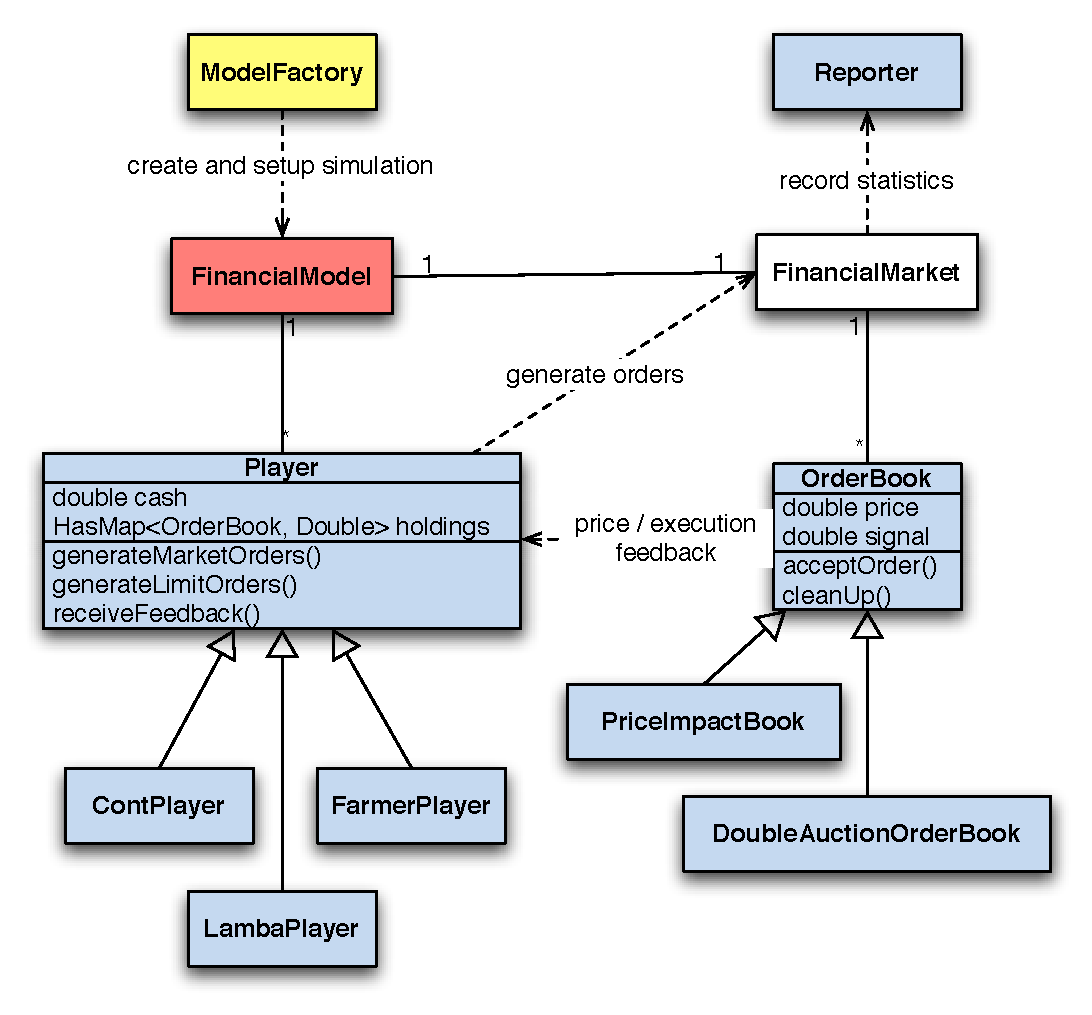
\includegraphics[width=1.0\textwidth]{../graphics/masterClassDiagram.pdf}
\caption{High-level UML class diagram of the main components and relations in the FinancialMarketModel, including the main attributes of Players and OrderBooks. Agent classes (light blue) inherit from the MASON \texttt{Steppable} interface while the master class is implementation of MASON's \texttt{SimState}.}
\label{fig:general_uml}
\end{figure}


\begin{figure}[htb]
\centering
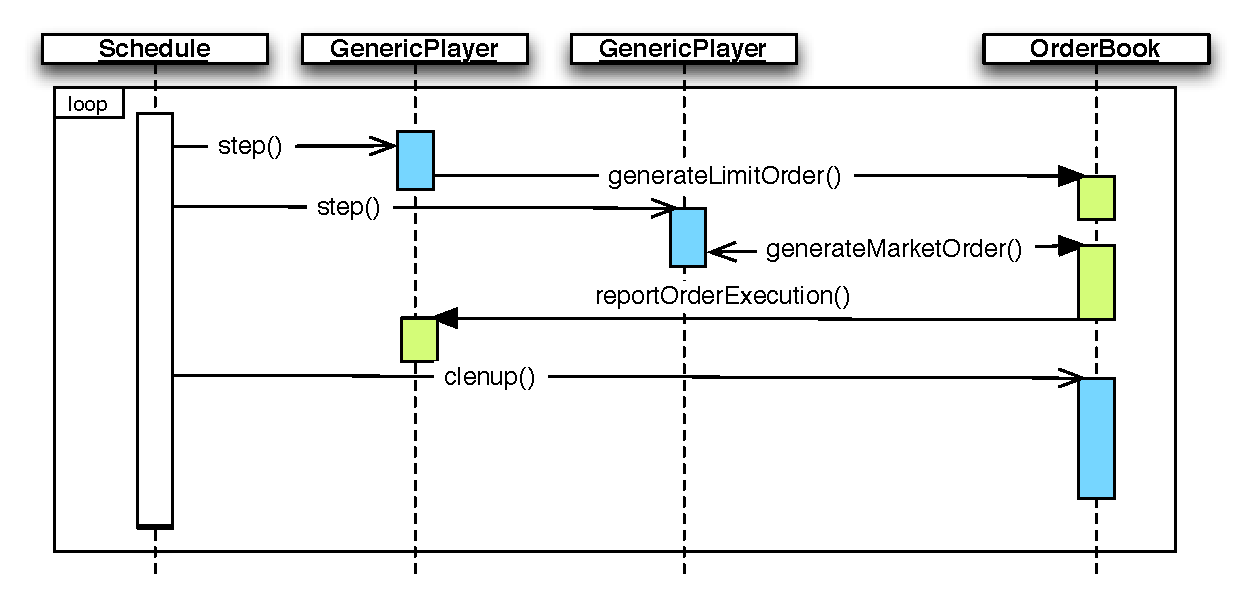
\includegraphics[width=1.0\textwidth]{../graphics/masterSequenceDiagram.pdf}
\caption{High-level UML sequence diagram of the interactions between main object of the FinancialMarketModel.}
\label{fig:general_uml}
\end{figure}


\section{Overview of Implemented Models}

\subsection{Cont Model}

The Cont model \cite{cont2006} is the simplest implemented. All traders (agents) follow the same behavioral rules. They are heterogeneous in the sense that they are given independently assigned (subjective) volatility thresholds $\theta_i(t)$. Each period, all agents recieve a common signal, which can be interpreted as public information or "news", in the form of IID Gaussian random variables $\epsilon_t$. Each agent $i$ responds to this signal by selling if $\epsilon_t < -\theta_i(t)$, buying if $\epsilon_t > \theta_i(t)$, and otherwise sitting out the period. The market then determines the excess demand and arrives at the market clearing price by means of a market impact function. Lastly, with probability $s$, agents update their threshold to match the absolute value of the return rate for the current period. Somewhat surprisingly, even this very simple "zero intelligence" model of agent behavior yields fairly realistic market movements, as presented on Figure \ref{fig:sampleDynamicsCont}.

TODO Note:cyclicality.

\begin{figure}[htbp]
  \begin{center}
   \mbox{
      \subfigure[Ask and bid prices.]{\scalebox{0.5}{\quad \quad 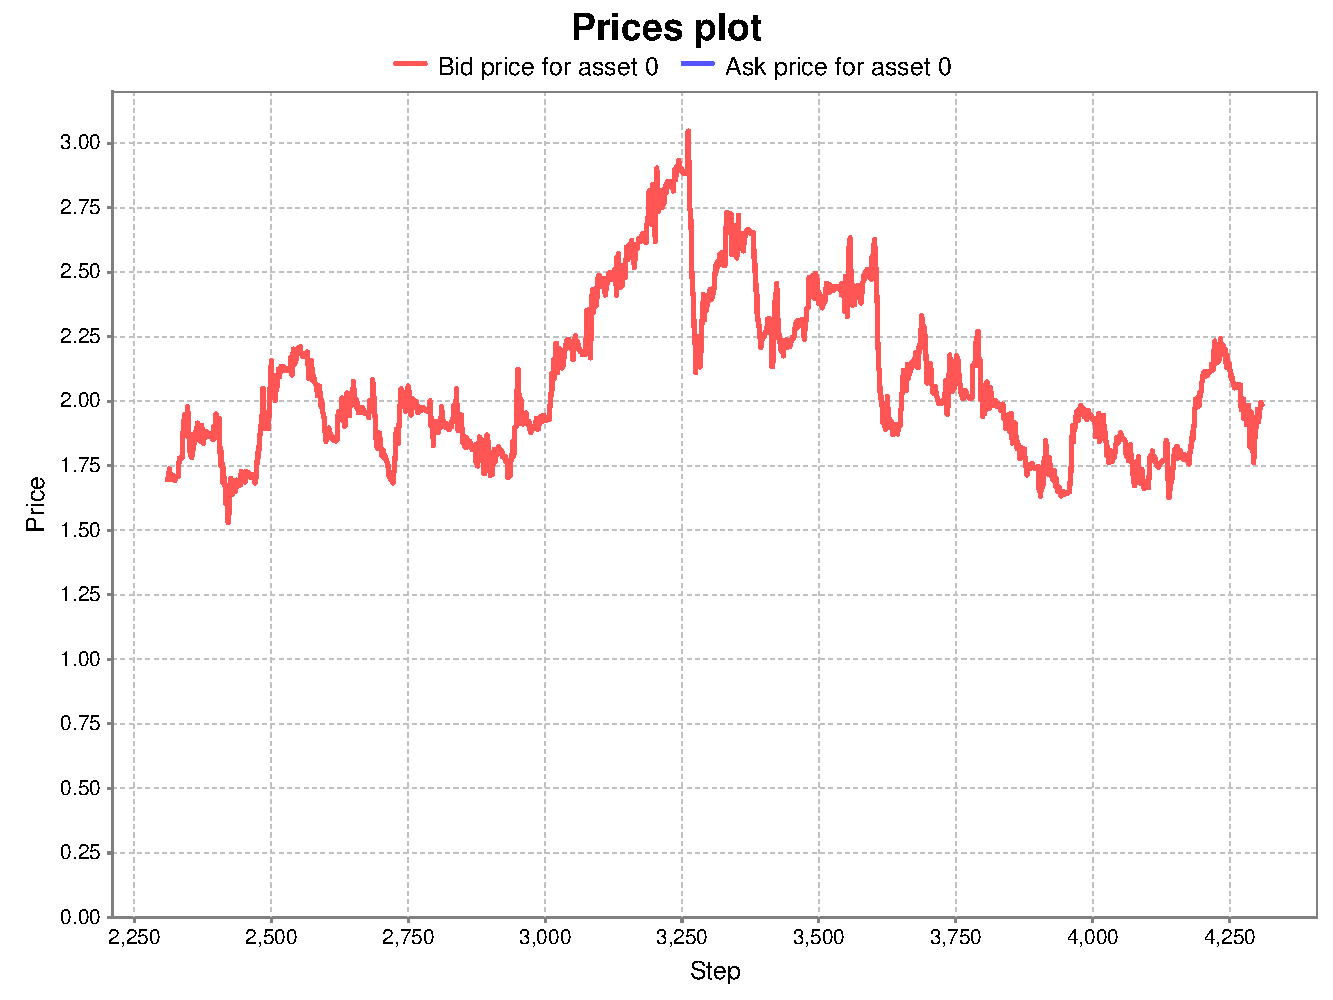
\includegraphics[width=0.9\textwidth]{../graphics/Cont-pricesPlot.pdf}}} \quad
      \subfigure[Raw and absolute returns.]{\scalebox{0.5}{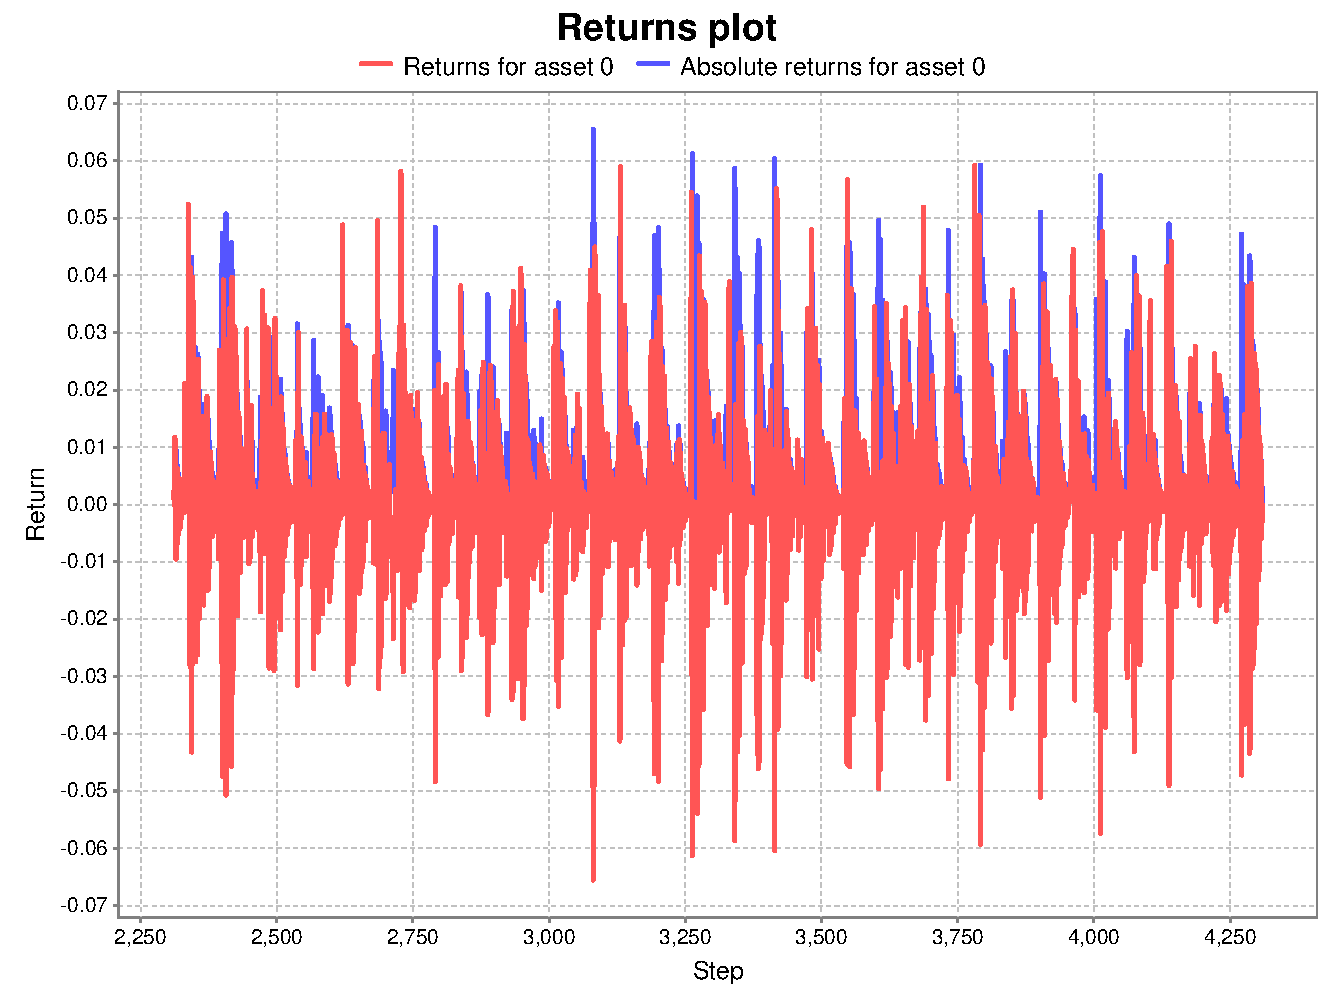
\includegraphics[width=1.00\textwidth]{../graphics/Cont-returnsPlot.pdf}}}
      }
    \mbox{
      \subfigure[Trade volumes.]{\scalebox{0.5}{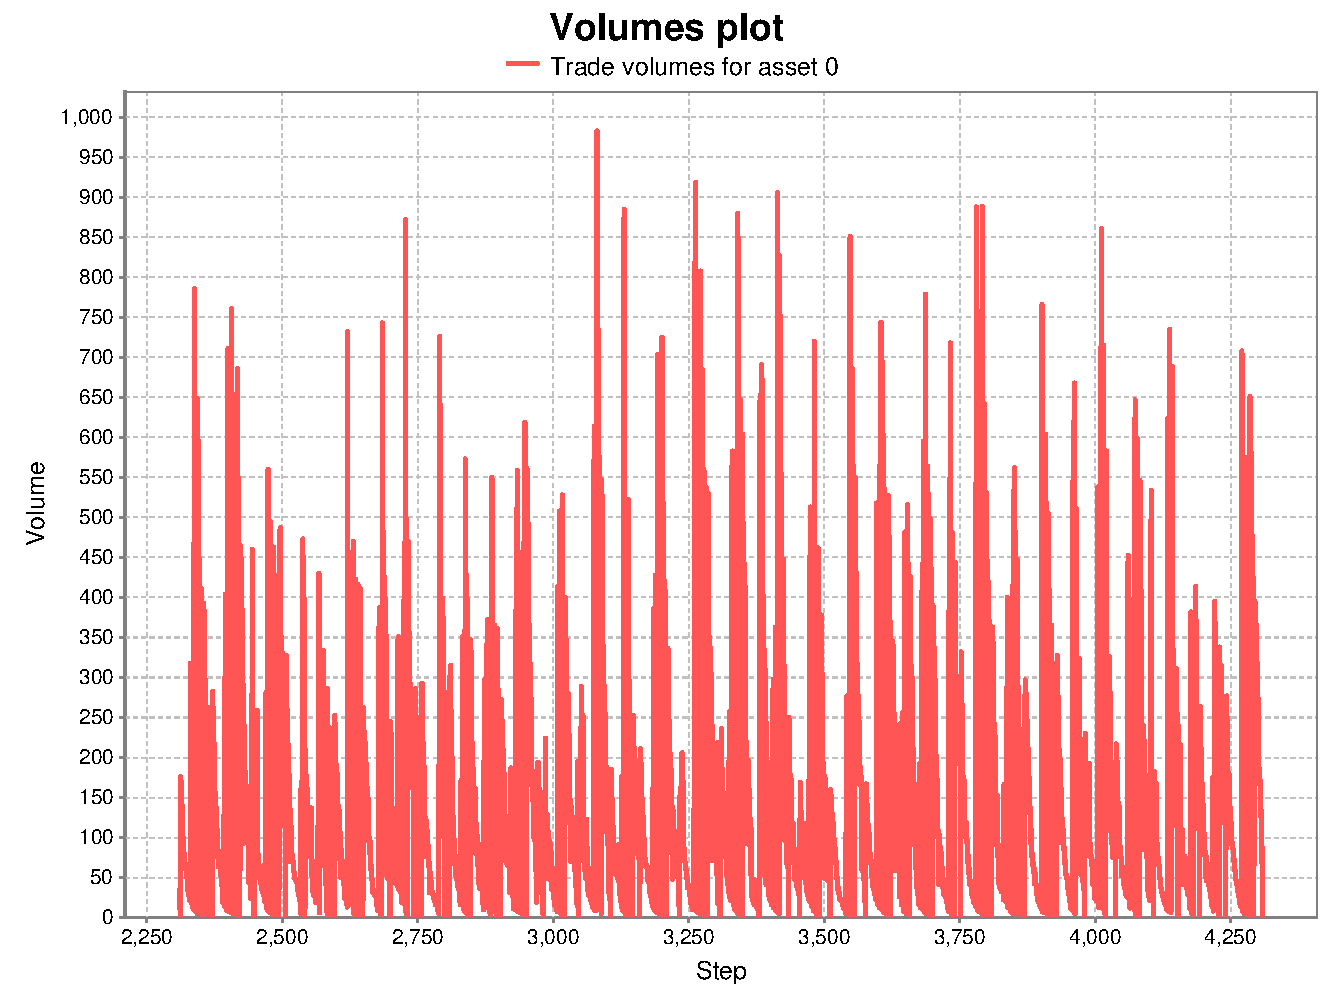
\includegraphics[width=1.00\textwidth]{../graphics/Cont-volumesPlot.pdf}}}
      }
    \mbox{
      \subfigure[Returns histogram.]{\scalebox{0.5}{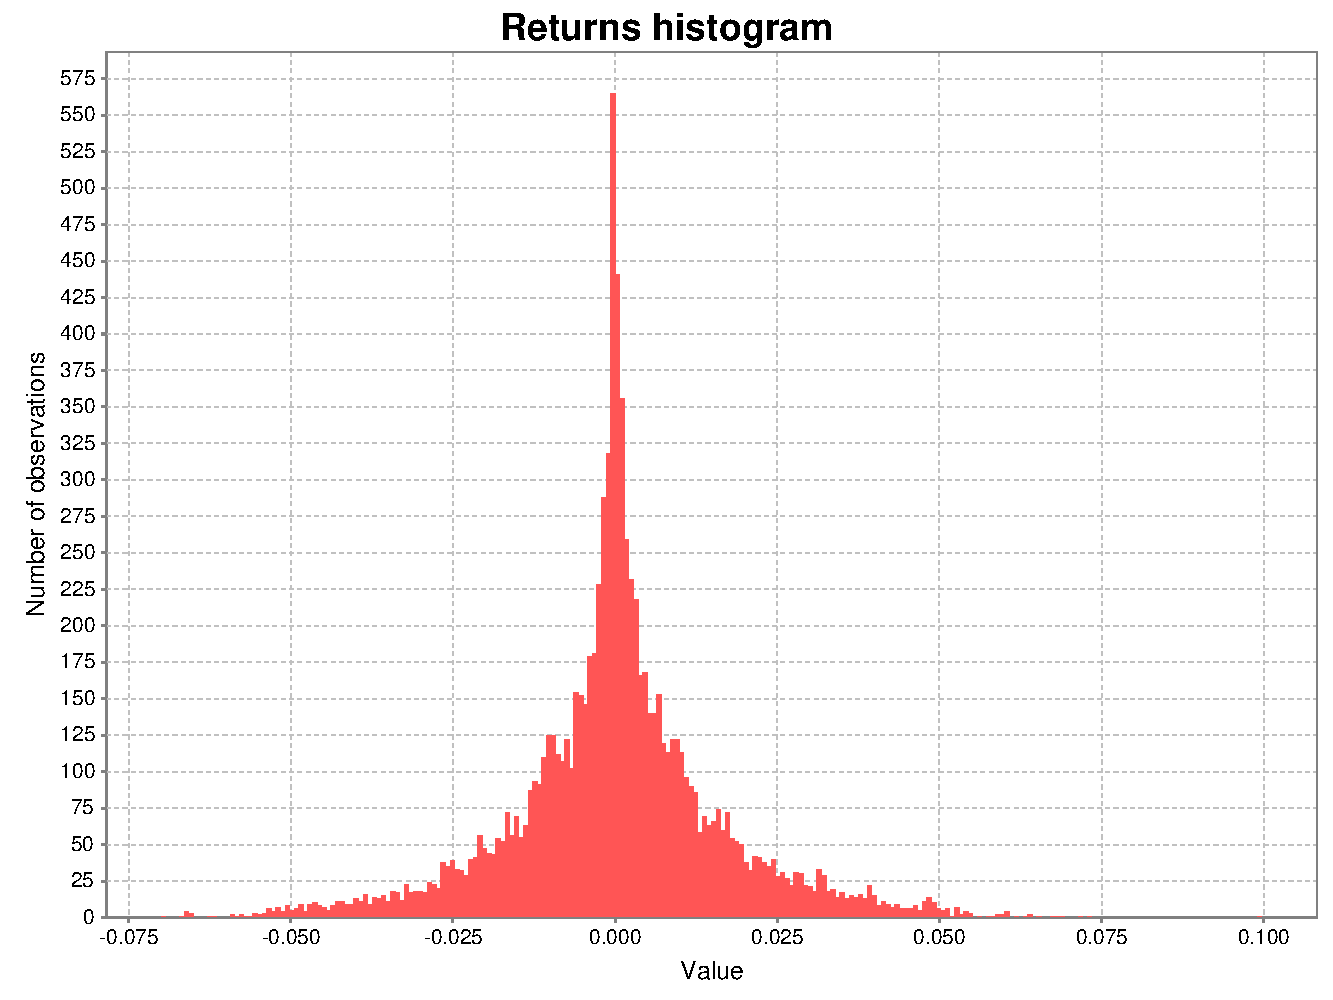
\includegraphics[width=1.00\textwidth]{../graphics/Cont-returnsHistogram.pdf}}} \quad
      \subfigure[Autocorrelation of returns.]{\scalebox{0.5}{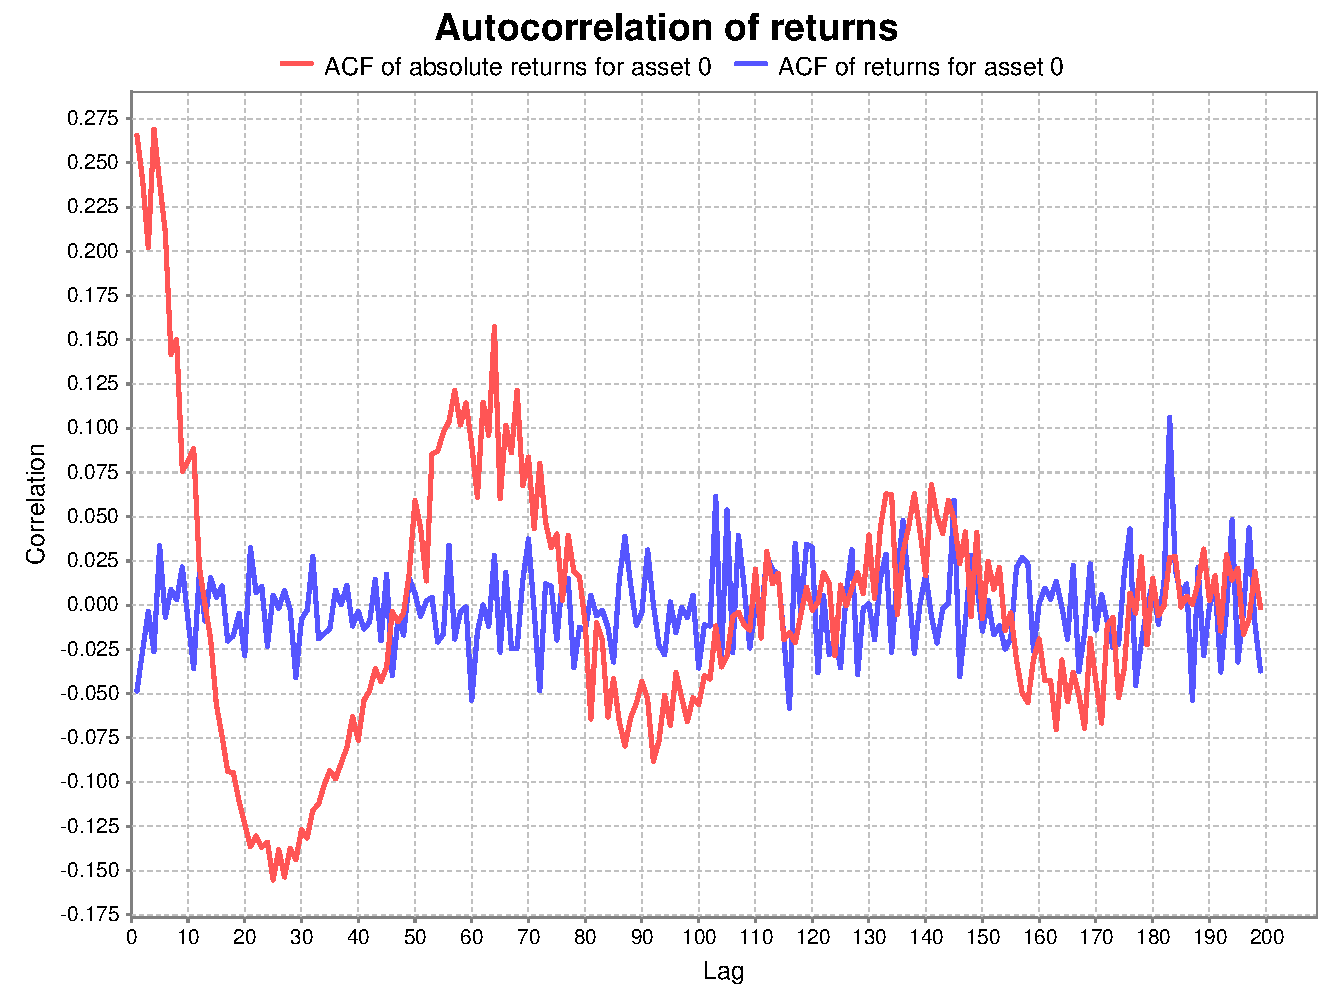
\includegraphics[width=1.00\textwidth]{../graphics/Cont-acfPlot.pdf}}}
      }
    \caption{Examples of outputs and statistics from a single run of the FinancialModel simulation for default Cont's parametrization.}
    \label{fig:sampleDynamicsCont}
  \end{center}
\end{figure}

\subsection{Farmer Model}
The Farmer model \cite{farmer2003} has two types of agents, which trade a single asset by means of a continuous double auction similar to those normally used on stock markets. "Patient" traders place orders place limit orders, which specify both a price and quantity they wish to buy or sell. Limit orders do not execute immediately, and may be canceled at any time. "Impatient" traders place market orders, specifying only a quantity, which execute immediately at the current best price, assuming there is sufficient liquidity provided by outstanding limit orders. This model also has simple behavioral logic for traders. Behavior is regulated by:
\begin{itemize}
\item Patient agents place limit orders of constant size at a Poisson rate per unit time, and with a randomly generated price. Orders are equally likely to be either buy or sell orders. Buy limit orders are placed uniformly anywhere in the semiinfinite interval below the current ask price ($-\infty < p < a(t)$), where $p$ is the \emph{logarithm} of the price; similarly for sell orders. A uniform distribution in log prices is equivalent to an exponential distribution in prices. In addition, outstanding limit orders are cancelled at a Poisson rate per unit time. All of these processes are independent.
\item Impatient agents place market orders of constant size at a Poisson rate per unit time.
\item A double auction order book. This manages the pending limit orders and facilitates trades between market and limit orders. It also provides aggregate market information such as return rate per unit time and bid-ask spreads.
\end{itemize}
This model explains a large portion of the spread and price diffusion of actual stocks given an order flow rate, which essentially means that the double auction structure has a large impact on the nature of market movements. The model also yields market behavior qualitatively close to actual markets in many respects, see Figure \ref{fig:sampleDynamicsFarmer}.

TODO Note: log vs. non-log prices
TODO Note: effect of price granularity

\begin{figure}[htbp]
  \begin{center}
   \mbox{
      \subfigure[Ask and bid prices.]{\scalebox{0.5}{\quad \quad 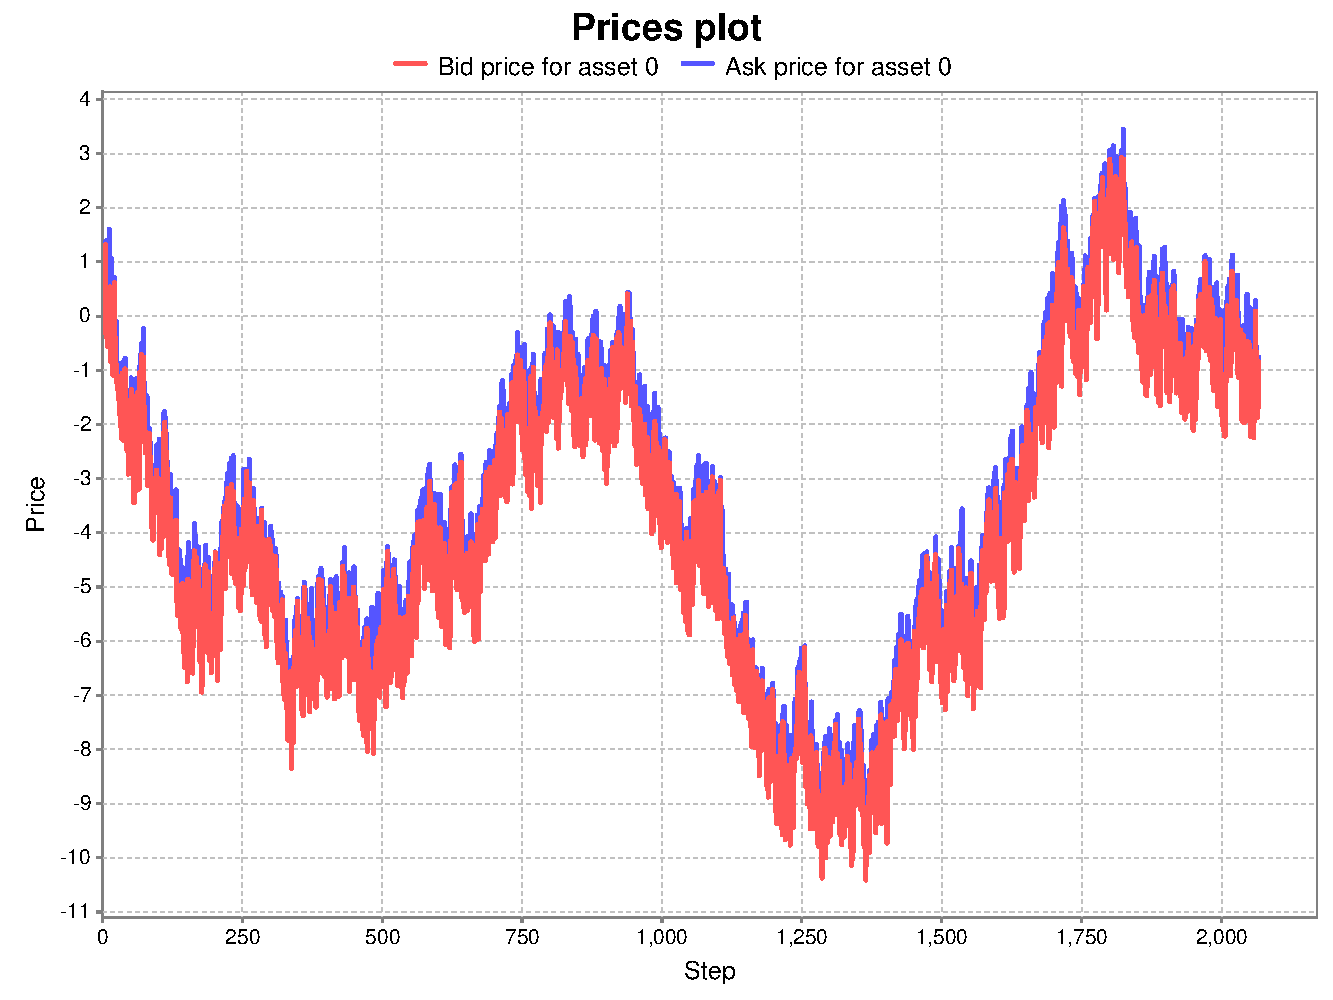
\includegraphics[width=0.9\textwidth]{../graphics/Farmer-pricesPlot.pdf}}} \quad
      \subfigure[Raw and absolute returns.]{\scalebox{0.5}{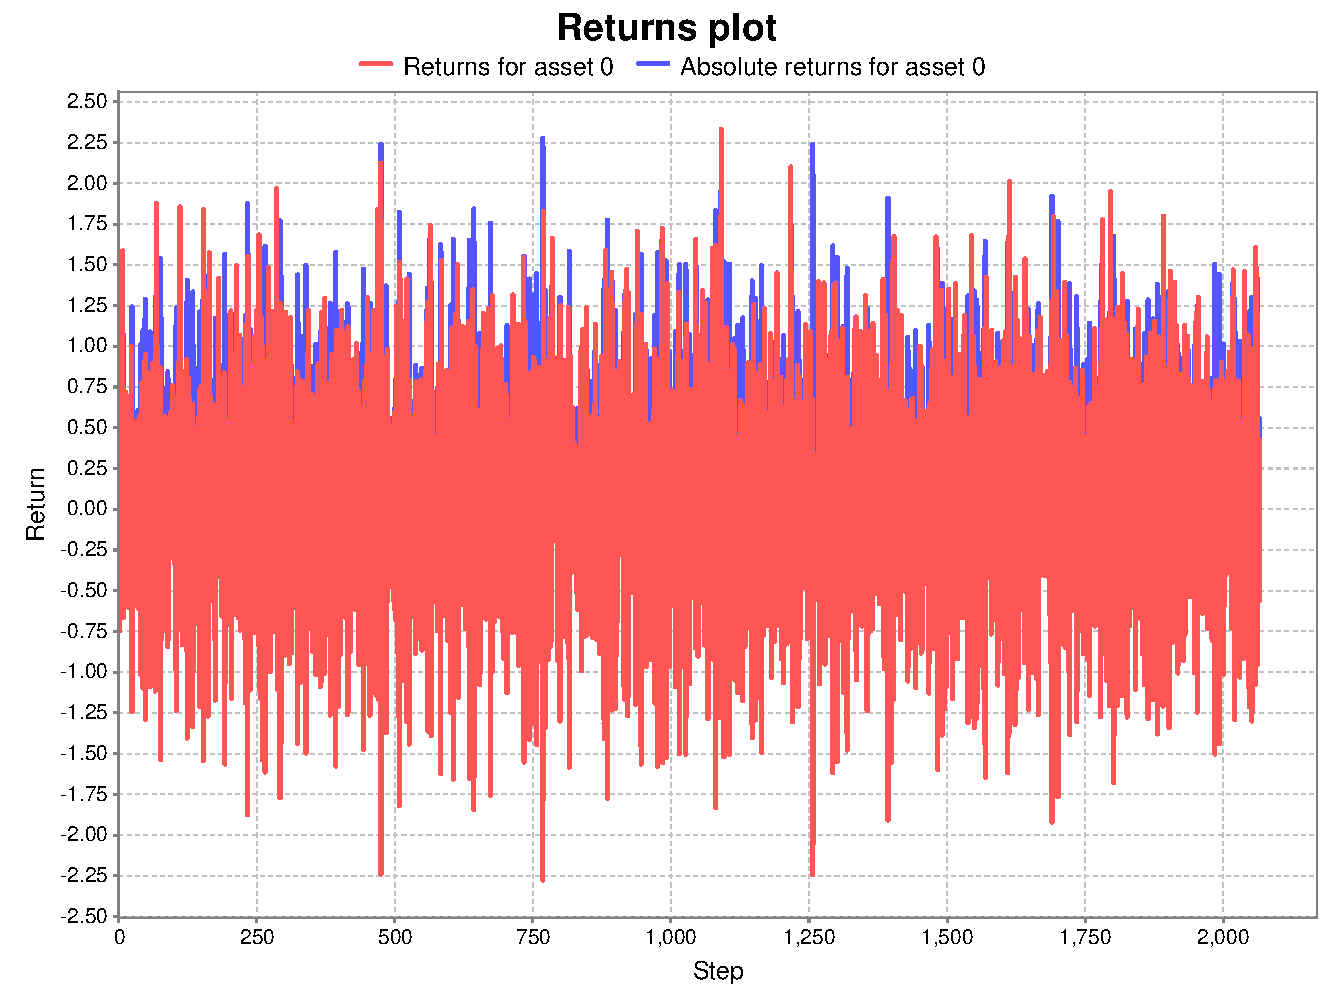
\includegraphics[width=1.00\textwidth]{../graphics/Farmer-returnPlot.pdf}}}
      }
    \mbox{
      \subfigure[Orderbook shape.]{\scalebox{0.5}{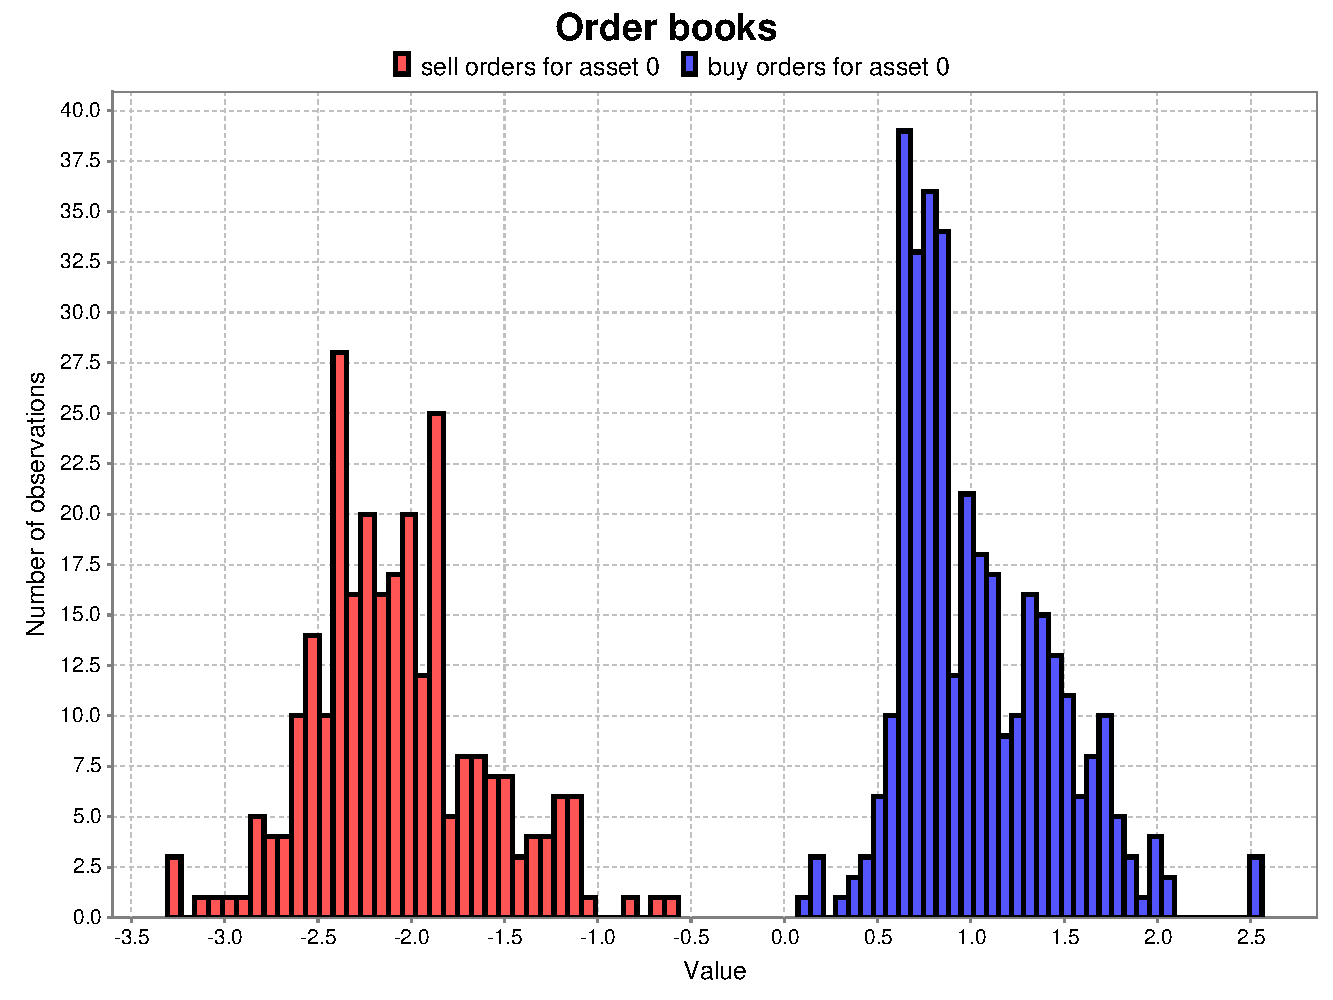
\includegraphics[width=1.00\textwidth]{../graphics/Farmer-orderbooks.pdf}}} \quad
      \subfigure[Trade volumes.]{\scalebox{0.5}{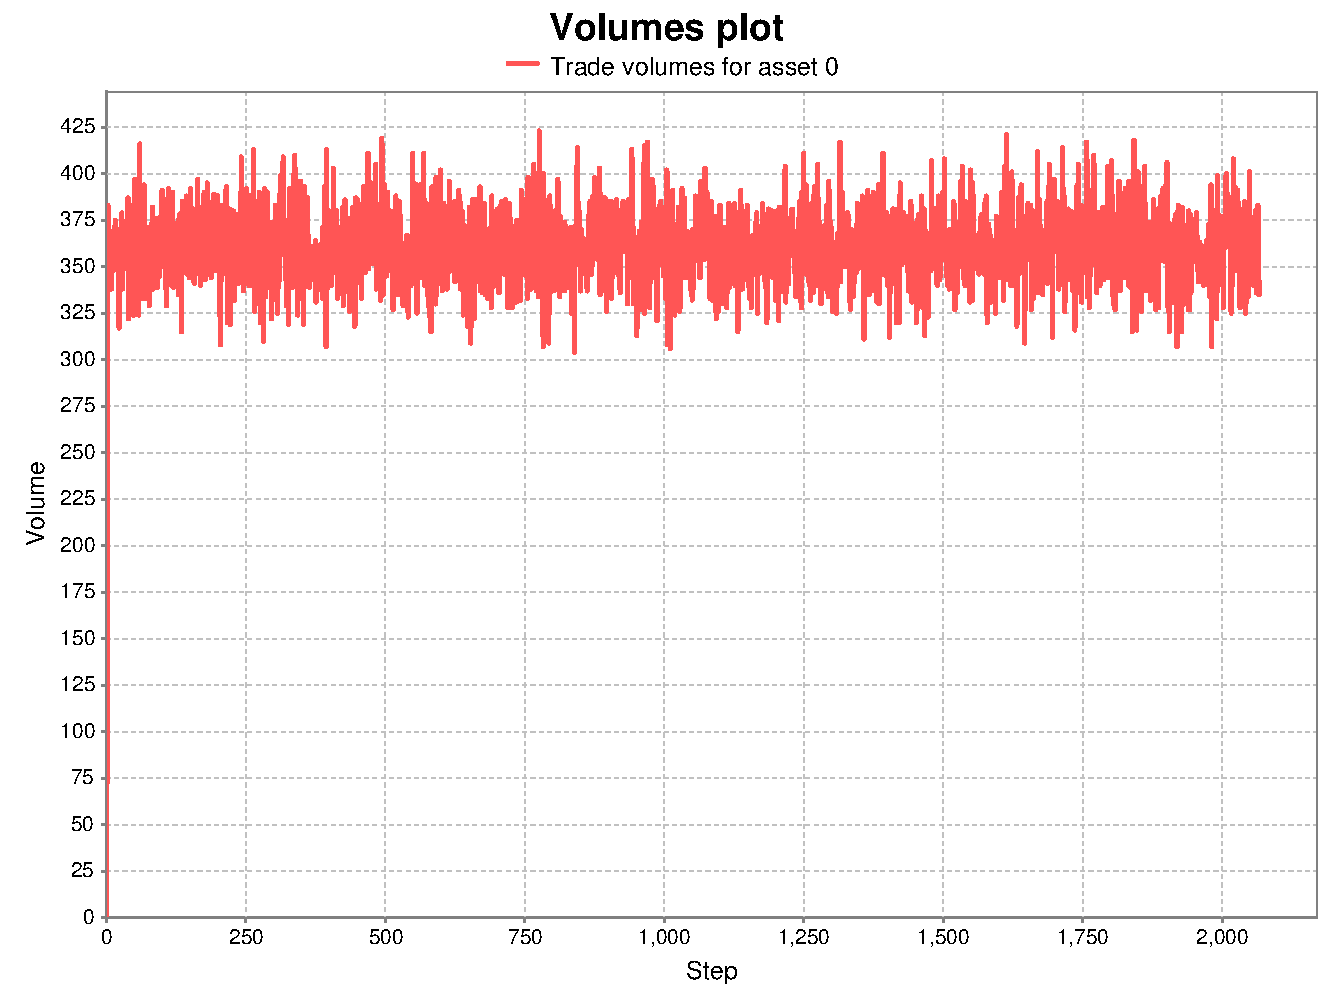
\includegraphics[width=1.00\textwidth]{../graphics/Farmer-volumesPlot.pdf}}}
      }
    \mbox{
      \subfigure[Returns histogram.]{\scalebox{0.5}{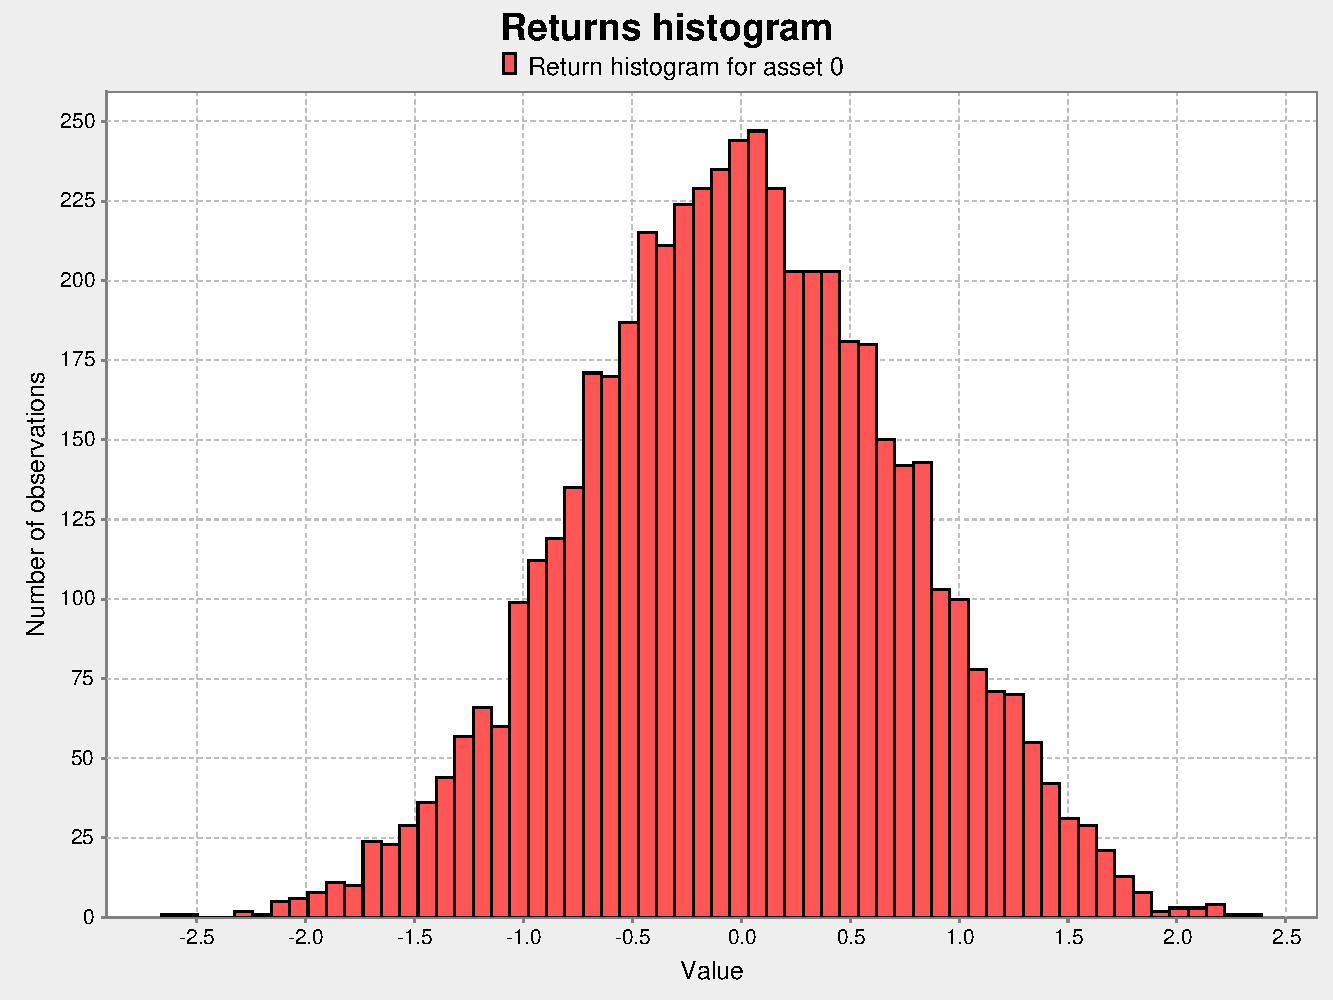
\includegraphics[width=1.00\textwidth]{../graphics/Farmer-returnsHistogram.pdf}}} \quad
      \subfigure[Autocorrelation of returns.]{\scalebox{0.5}{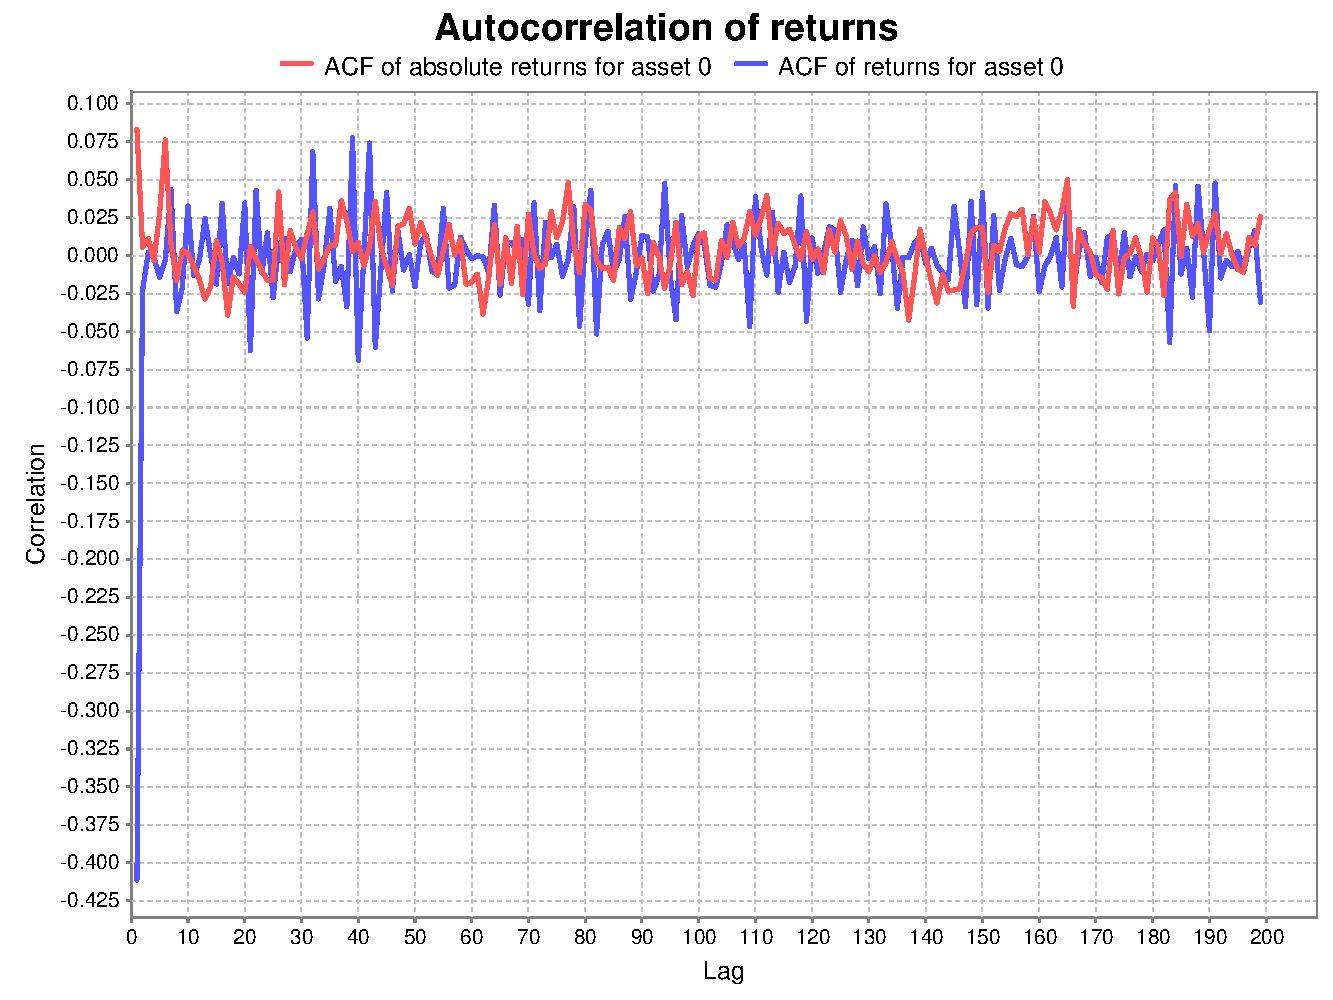
\includegraphics[width=1.00\textwidth]{../graphics/Farmer-acfReturns.pdf}}}
      }
    \caption{Examples of outputs and statistics from a single run of the FinancialModel simulation for default Farmer's parametrization.}
    \label{fig:sampleDynamicsFarmer}
  \end{center}
\end{figure}

\subsection{Farmer-Cont Model}
We constructed a model combining aspects of the Farmer model with aspects of the Cont model. The result is a model which is still essentially zero intelligence, but which exhibits empirically positive characteristics of both models. In this model there are two types of agents, which interact via the continuous double auction mechanism, as in Farmer. In fact, the Patient traders, which place limit orders and thus provide liquidity, remain the same. Impatient traders are modeled after Cont. They have heterogeneous volatility thresholds, and place market orders depending upon how public information in the form of a normally distributed random variable compares with these thresholds.
TODO Show results.
TODO Note: liquidity issues



\section{Verification of Correctness}
TODO: show results side by side with original papers' figures
\bibliographystyle{plainnat}
\bibliography{master}

\end{document}

%%%%%%%%%%%%%%%%%%%%%%%%%%%%%%%%%%%%%%%%%%%%%%%%%%%%%%%%%%%%%%%%%%%%%%
%% The end.
%%%%%%%%%%%%%%%%%%%%%%%%%%%%%%%%%%%%%%%%%%%%%%%%%%%%%%%%%%%%%%%%%%%%%% 
